\section{Browserumgebung}

\textit{Hier soll eine Beschreibung der Umgebung erstellt werden, mit Nennung der speziellen Eigenschaften (Keywords: Sandbox, CORS, Logging)}

Als JavaScript 1997 veröffentlicht und in den NetScape Navigator integriert wurde, gab es die berechtigen Bedenken, dass das Öffnen einer Webseite dem Betreiber erlaubt Code auf dem System eines Nutzers auszuführen. Damit dies nicht eintritt, wurde der JavaScript Ausführungskontext in eine virtuelle Umgebung  integriert - einer sogenannten Sandbox. \cite{LearningJavaScript}

Zusätzlich hierzu gibt es weitere Einschränkungen, welche definieren was für Daten innerhalb der JavaScript Umgebung abgerufen werden dürfen und mit welchen Diensten kommuniziert werden darf \cite{LearningJavaScript}. Zwei wichtige dieser Einschränkungen werden folgend erklärt.

\subsection{Content-Security-Policy}

Content-Security-Policy definiert, welche Ressourcen (also Bilder, Skripte, etc.) von der Webapplikation aus geladen werden dürfen und über welches Protokoll. Dies dient dem Schutz vor cross-site scripting (XSS), indem eine Webapplikation beschränken kann, welche Aufrufe von ihr aus getätigt werden dürfen. Wird beispielsweise eine JavaScript-Bibliothek aus einem externen CDN benutzt und die Bibliothek wird zu späterer Zeit böswillig ausgetauscht oder modifiziert, kann durch die Härtungsmaßnahme einer Content-Security-Policy gewährleistet werden, dass keine Daten an unbekannte Server geschickt werden dürfen \cite{MDNContentSecurityPolicy}.

\subsection{Cross-Origin Resource Sharing (CORS)}

\section{JavaScript-basierte Webapplikationen}
% \textit{Hier soll beschrieben werden, was JavaScript-basierte Webapplikationen sind.}

% Diese Ausarbeitung konzentriert sich, wie im Titel beschrieben, auf JavaScript-basierte Webapplikationen. Weiterhin wird sich auf sogenannte Single-Page-Applications (SPAs) konzentriert, welche eine Submenge der JavaScript-basierten Webapplikationen darstellen. Um allen Lesern eine gleiche Grundkenntnis zu ermöglichen, werden diese Konzepte nun kurz vorgestellt.

%In diesem Abschnitt wird erläutert, mit welcher der Art von Anwendungen sich diese Arbeit beschäftigt und welche Eigenschaften diese besitzen.

\subsection{JavaScript-basierte Webapplikationen}

Eine JavaScript-basierte Webapplikation, ist eine Webapplikation, in der die Hauptfunktionalitäten über JavaScript realisiert werden. Dies umfasst unter anderem Interaktivität und dynamische Inhaltsdarstellung. Hierbei werden meist nur Grundgerüste in HTML und gegebenenfalls auch CSS bereitgestellt, und die eigentlichen Inhalte werden dynamisch mit JavaScript erstellt. Die Inhalte werden überwiegend über zusätzliche Schnittstellen der Webapplikation bereitgestellt.

\subsection{Single-Page-Applications}

Single-Page-Applications (SPAs) sind eine Submenge der JavaScript-basierten Webapplikationen und gehen bei der dynamischen Inhaltsdarstellung einen Schritt weiter. Logische Seiten werden nicht über eigene HTML-Dateien bereitgestellt, sondern dynamisch von der Anwendung aus erzeugt. Für das Bereitstellen einer solchen Applikation, ist daher nur ein simpler Webserver nötig und ein oder mehrere Dienste, von dem die SPA ihre Inhalte abrufen kann. Populäre Frameworks, um SPAs zu Erstellen, sind beispielsweise Angular \cite{AngularHomepage}, React \cite{ReactHomepage} oder Vue.js \cite{VueJSHomepage}.

In dieser Arbeit werden SPAs untersucht, denn einerseits fallen diese in das Interessengebiet und das aktuelle Projektumfeld der Open Knowledge, anderseits gibt es aber auch einige Eigenheiten, die die Nachvollziehbarkeit reduzieren. Beispielsweise gehen durch die starke Trennung von Client und Server auch Kontextinformationen verloren. Zudem wird die Applikation beim Client größer und komplexer, welches mit einem erhöhten Potenzial für Ungereimtheiten einher geht.
	
\newpage

% \section{Instandhaltung und Support}

\section{Softwarebetrieb}

Diese Arbeit konzentriert sich auf Software, die sich in der Betriebsphase befindet. Gängige Software-Entwicklungszyklen und ihre Definition dieser Phase werden folgend beschrieben.

\subsection{Klassisches Vorgehen}

	\begin{wrapfigure}[14]{r}{0.45\linewidth}
		\centering
		\vspace{-\baselineskip}
		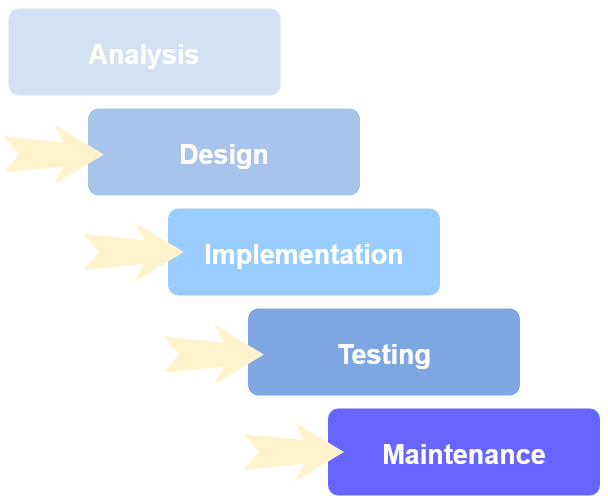
\includegraphics[width=\linewidth]{img/02_theorie/software-life-cycle.png}
		\caption{Lebenszyklus einer Software}
		\label{fig:software-development-life-cycle}
		\source{Eigene Darstellung von \cite{ASimulationModelWaterfallSoftware}}
	\end{wrapfigure}
	
	In vielen Modellen über den Lebenszyklus einer Software wird die Phase während der Betreibung oftmals \enquote{Maintenance} genannt \cite{ManagingTheComplexityOfWebSystemsDevelopment} \cite{ASimulationModelWaterfallSoftware}, in der Instandhaltung und Support den Alltag bestimmen. Sie ist nach Zelkowitz \etal \cite{PrinciplesOfSoftwareEngineeringAndDesign} für rund zwei Drittel der Entwicklungskosten verantwortlich, begründet durch exponentielle Steigung \cite{ExtremeProgrammingExplained}.
	
	Das Wasserfallmodell \cite{ASimulationModelWaterfallSoftware} sowie das V-Modell XT \cite{WaterfallVsVModelVsAgile} sehen vor, dass in dieser Phase die Software funktionstüchtig gehalten wird und dass die Anforderungen an die Software erfüllt sind. Bei nicht-erfüllten Anforderungen oder Fehlern, werden diese behoben. Jedoch ein kontinuierlicher Verbesserungsprozess ist in dieser Phase nicht vorgesehen.
	
%	Es werden immer bessere Methoden entwickelt, um Probleme in Software - oder auch Bugs - zu verringern. Jedoch erhöht sich zugleich die Komplexität von Software, was zur Ursache hat, dass es mehr Nährboden für Bugs gibt \cite{TrackingDownSoftwareBugsAnomalyDetection}. De-facto sind Bugs ein unvermeidbarer Bestandteil einer Software und müssen daher erwartet und gehandhabt werden \cite{TheMythicalManMonth}.
%	
%	Wenn nun ein Bug auffällt, sei es durch einen Nutzer oder auch zufällig einem Stakeholder, muss entschieden werden, ob dieser zu beheben ist. Wenn eine Behebung angestrebt wird, benötigt der Stakeholder meistens Rahmeninformationen \cite{WhatMakesAGoodBugReport} um den Bug ggf. zu reproduzieren und die Situation nachzuvollziehen. Desto mehr Verständnis der Stakeholder über das Problem erhält, desto schneller und präziser kann er die Ursache aufdecken. Die Ermöglichung der schnellen Verständnis über ein Problem, wird in dieser Arbeit \textbf{Nachvollziehbarkeit} genannt.

\subsection{Agiles Vorgehen}

	\begin{wrapfigure}[11]{l}{0.45\linewidth}
		\centering
		\vspace{-\baselineskip}
		\includegraphics[width=\linewidth]{img/02_theorie/devops-life-cycle.png}
		\caption{DevOps Toolchain}
		\label{fig:devops-life-cycle}
		\source{Wikimedia Commons \cite{DevOpsLifeCycle}}
	\end{wrapfigure}
	
	Bei agilen Ansätzen wird der Betrieb meist nicht abgegrenzt von der normalen Entwicklung. In dieser Phase werden weiterhin Anforderungen erhoben und diese Stück für Stück umgesetzt \cite{WaterfallVsVModelVsAgile}. Vorteilhaft dabei ist, dass auf neue Wünsche oder Auffälligkeiten sehr einfach reagiert werden kann. Es wird eine kontinuierliche Verbesserung angestrebt.
	
	Um den kontinuierlichen Entwicklungs- und Deploymentprozess reibungslos ablaufen zu lassen, werden Ansätze wie DevOps \cite{DevOps} verfolgt (vgl. \autoref{fig:devops-life-cycle}).

\newpage

\section{Nachvollziehbarkeit}

	\textit{Hier soll die Nachvollziehbarkeit allgemein beschrieben werden und warum sie erstrebenswert ist.}

	Sie beschäftigt sich mit der Informationserfassung und -aufbereitung, um das Verhalten eines Systems und die Interaktionen der Nutzer für die Stakeholder verständlich zu machen. Sie ist getrennt von der Anstrebung einer Reproduzierbarkeit nach der wissenschaftlichen Methode anzusehen.
	
	{\color{red}\textit{\lipsum[1]}}
	
	Tritt ein Problem bei einem Nutzer auf, aber die Stakeholder erhalten nicht ausreichende Informationen, so kann der Bug ignoriert werden oder in Vergessenheit geraten. Dies geschah im Jahr 2013, als Khalil Shreateh eine Sicherheitslücke bei Facebook fand und bei Facebooks Bug-Bounty-Projekt Whitehat meldete \cite{FacebookBugBounyHunt}. Sein Fehlerreport wurde aufgrund mangelnder Informationen abgelehnt:
	
	\begin{quotation}
	Unfortunately your report [...] did not have enough technical information for us to take action  on  it. We  cannot  respond  to  reports  which  do  not contain enough detail to allow us to reproduce an issue.
	\end{quotation}

\subsection{Nachvollziehbarkeit bei Webapplikationen}

	\textit{Hier sollen die Besonderen Hürden bei Webapplikationen hervorgehoben werden (indirekte Kommunikation, keinen Zugriff auf Logs, etc.)}

	\textit{Weiterhin soll beschrieben werden, }